\subsection{Le labyrinthe}
\label{subsec:labyrinthe}

% Pour chaque partie de l'implémentation du labyrinthe je pense présenter les fichiers .java (classes, interfaces, enums...) qui gèrent chaque secction de l'implémentation. En accompagnant chaque section d'une image de la partie pertinente du diagramme des classes.

\subsubsection{Le Modèle}
\label{subsubsec:modele}

Nous avons une interface \textbf{\textit{MazeModel}} avec son implémentation
\textbf{\textit{MazeModelImplementation}} qui servent à modéliser le Labyrinthe.
Afin de représenter le labyrinthe, nous avons utilisé une matrice de booléens
où '\textit{true}' représente un chemin et '\textit{false}' représente un mur.
% TODO: Ajouter une image du diagramme des classes de l'implémentation de l'interface \textbf{\textit{MazeModel}}' et de son implémentation '\textbf{\textit{MazeModelImplementation}}

Les labyrinthes sont générés grâce à un générateur qui est géré par
l'interface \textbf{\textit{BoardGenerator}}' et son implémentation '\textbf{\textit{DepthFirstGenerator}}.
L'algorithme de génération utilisé est le Randomized Depth-First Search.
% TODO: Ajouter une image du diagramme des classes de l'implémentation de l'interface \textbf{\textit{BoardGenerator}}' et de son implémentation '\textbf{\textit{DepthFirstGenerator}}

L'enum \textbf{\textit{GameMode}} permet de définir les différents modes de jeu.
Chaque type de jeu a sa propre implémentation de l'interface \textbf{\textit{GameModeData}}
qui sert à définir les données des paramètres de jeu
(taille, type de score, difficulté) et la classe \textbf{\textit{GameData}} se charge de
regrouper ces données avec la liste des joueurs.
% TODO: Ajouter une image du diagramme des classes de l'implémentation de l'enum \textbf{\textit{GameMode}}' avec son implémentation '\textbf{\textit{GameModeData}}' et de la case '\textbf{\textit{GameData}}

Les labyrinthes sont créés grâce aux méthodes de la classe
\textbf{\textit{MazeModelFactory}} qui se charge de mettre à disposition des méthodes
qui permettent de créer des labyrinthes de différentes tailles selon les modes
de jeu.
% TODO: Ajouter une image du diagramme des classes de l'implémentation de la classe \textbf{\textit{MazeModelFactory}}

En ce qui concerne les joueurs, nous avons une interface \textbf{\textit{Player}} avec son
implémentation \textbf{\textit{PlayerImplementation}} qui permettent de représenter un
joueur. Ces derniers sont caractérisés par un nom, une couleur, des coordonnées, un
statut, un nombre de mouvements et un temps qui correspond au temps pris pour finir le labyrinthe.
Ces deux dernières données servent à calculer le score d'un joueur.
%TODO : Ajouter une image du diagramme des classes de l'implémentation de l'interface \textbf{\textit{Player}}' et de son implémentation '\textbf{\textit{PlayerImplementation}}

Pour pouvoir calculer le score des joueurs, nous avons plusieurs éléments qui
utilisent les données évoquées précédemment. L'interface \textbf{\textit{ScoreCalculator}}
et ses implémentations permettent de calculer le score d'un joueur à partir
d'une implémentation de \textbf{\textit{ScoreInfo}} qui stocke les informations
nécessaires. La classe \textbf{\textit{ScoreCalculatorFactory}} se charge de créer des
instances d'implémentations de \textbf{\textit{ScoreCalculator}} en fonction du type de
score et des informations selon le type de score (respectivement grâce à l'enum
\textbf{\textit{ScoreType}}, et \textbf{\textit{ScoreInfo}}). Le calcul du score se fait
mathématiquement en fonction du nombre de mouvements, du temps passé et de la
difficulté du labyrinthe.
% TODO : Ajouter une image du diagramme des classes de \textbf{\textit{ScoreCalculator}}' et de ses implémentations, de '\textbf{\textit{ScoreCalculatorFactory}}', de l'enum '\textbf{\textit{ScoreType}}' et de '\textbf{\textit{ScoreInfo}}

L'enum \textbf{\textit{Direction}} permet de définir les quatre directions de déplacements.
% TODO : Ajouter une image du diagramme des classes de l'enum \textbf{\textit{Direction}}
\subsubsection{La Vue}
\label{subsubsec:vue}

Pour l'implémentation de la Vue, nous avons choisi d'utiliser les librairies \textbf{SWING} et \textbf{AWT}
\subsubsection{Les Contrôleurs}
\label{subsubsec:controleur}

Afin de garantir le bon fonctionnement de notre application, nous avons implémenté un contrôleur qui permet de gérer les interactions entre les différentes parties de notre application. Le contrôleur est composé de plusieurs classes qui permettent de gérer les différents menus, les paramètres audio, les règles du jeu, la création de partie, la partie en elle-même, etc. C'est ce qui lie notre MVC et permet de faire fonctionner notre application.

\paragraph{Les mouvements}

Nous avons décidé de créer une interface \textbf{\textit{MazeController}} qui est implémentée par \textbf{\textit{MazeControllerImplementation}}. Cette interface
contient toutes les méthodes qui permettent de gérer les mouvements du joueur.


Pour déplacer les joueurs nous utilisons principalement la voix, mais nous donnons aussi au jouer le choix d'utiliser le clavier. Pour gérer ces deux types de mouvements
nous utilisons deux classes:
\begin{itemize}
    \item \textbf{\textit{VoiceMovementController}} qui permet de gérer les mouvements du joueur avec la voix
    \item \textbf{\textit{KeyboardMovementCOntroller}} qui permet de gérer les mouvements du joueur avec le clavier
\end{itemize}
Ces deux classes sont utilisées en composition dans la classe \textbf{\textit{MazeControllerImplementation}} qui permet de gérer les mouvements du joueur.


\paragraph{Les menus}

Afin de gérer la fenêtre de notre jeu et de naviguer entre les différents menus, nous avons créé la classe \textbf{\textit{MenuFrameHandler}}. Cette classe se charge de changer le \textbf{\textit{JPanel}} de la fenêtre principale de notre application, qui est une \textbf{\textit{JFrame}}.


\paragraph{L'écran d'accueil} (\ref{fig:StartMenu})

Nous avons un écran d'accueil, géré par la classe \textbf{\textit{StartMenu}}, qui possède des boutons pour:

\begin{itemize}
    \item Aller au menu de création de partie
          \vcenteredinclude[height=5mm]{ressources/Implementation/Labyrinthe/Controleur/StartButton.png}
    \item Aller au menu des paramètres audio
          \vcenteredinclude[height=5mm]{ressources/Implementation/Labyrinthe/Controleur/Settings.png}
    \item Afficher les règles du jeu
          \vcenteredinclude[height=5mm]{ressources/Implementation/Labyrinthe/Controleur/QuestionMark.png}
          %   \item Afficher les crédits
          % \item Quitter le jeu
\end{itemize}

Les différents éléments graphiques tels que le GIF et les images des boutons sont gérés par la classe \textbf{\textit{JPanelWithImages}}.

\begin{figure}[h!]
    \centering
    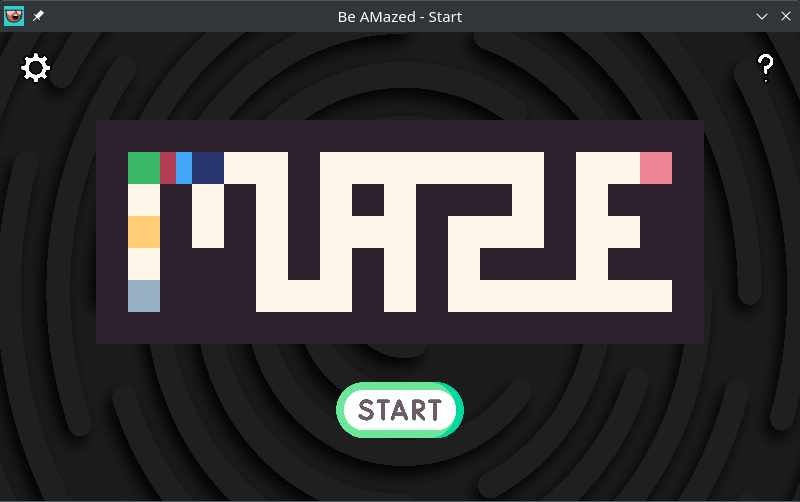
\includegraphics[width=10cm]{ressources/Implementation/Labyrinthe/Controleur/StartMenu.png}%
    \caption{L'écran d'accueil}
    \label{fig:StartMenu}
\end{figure}
\FloatBarrier

\paragraph{Les paramètres audio} (\ref{fig:Rules})

La vue des paramètres audio sera abordée dans la section \ref{subsec:son}.

\paragraph{Les règles de jeu}

Les règles du jeu sont affichées en anglais dans une fenêtre qui se superpose à celle du menu principal.

\begin{figure}[h!]
    \centering
    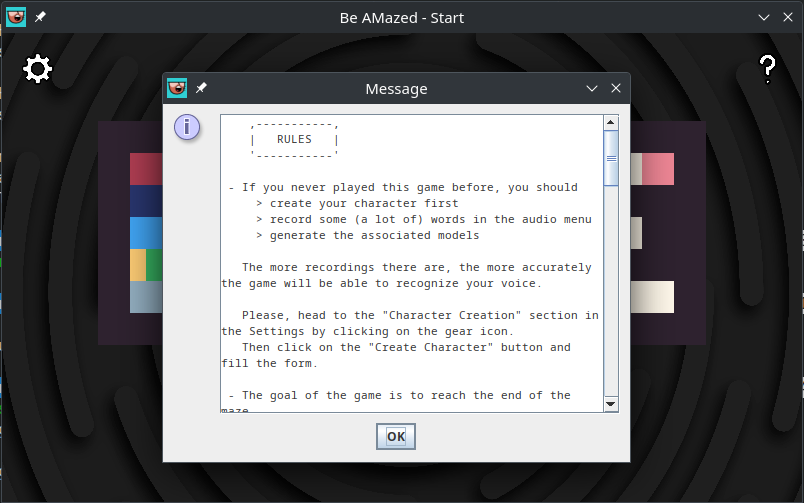
\includegraphics[width=10cm]{ressources/Implementation/Labyrinthe/Controleur/Rules.png}%
    \caption{Les règles du jeu}
    \label{fig:Rules}
\end{figure}
\FloatBarrier

\paragraph{La création de partie}

La création de la partie se décompose en plusieurs étapes et dispose de plusieurs éléments graphiques afin de permettre à l'utilisateur de choisir les paramètres de la partie qu'il souhaite jouer (nombre de joueurs, difficulté, etc.) le plus facilement possible. Cela est rendu possible par la classe \textbf{\textit{SettingsMenu}} qui gère l'ensemble des menus de paramétrage de la partie.

\subparagraph*{Le choix du mode de jeu} (\ref{fig:ModeSelection})

Le menu déroulant permet de choisir entre les différents modes de jeu disponibles. Il est géré par la classe \textbf{\textit{SelectionPanel}}.

\begin{figure}[h!]
    \centering
    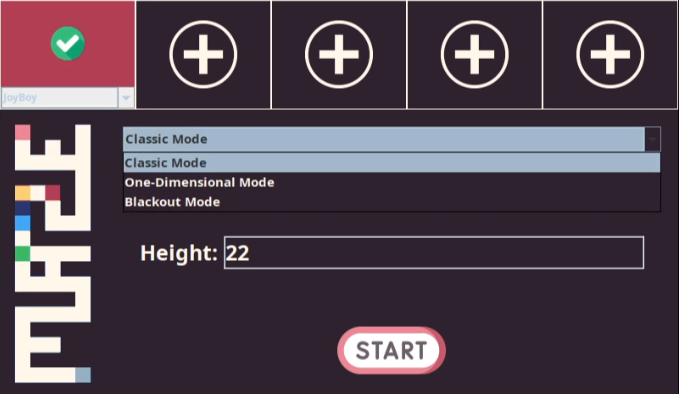
\includegraphics[width=10cm]{ressources/Implementation/Labyrinthe/Controleur/SettingsMenu_ModeList.png}%
    \caption{Menu déroulant des modes de jeu}
    \label{fig:ModeSelection}
\end{figure}
\FloatBarrier

Pour les afficher les menus des différents modes de jeu, nous avons des classes qui permettent de gérer les différents panels concernés. Ces classes sont des implémentations de l'interface  \textbf{\textit{PanelHandler}} et sont créées grâce à la classe  \textbf{\textit{PanelHandlerFactory}}.

\subparagraph*{Le mode Classique} (\ref{fig:ClassicMode})

Grâce à la classe \textbf{\textit{ClassicPanelHandler}}, nous avons à disposition deux entrées texte permettant de choisir la taille du labyrinthe.

\begin{figure}[h!]
    \centering
    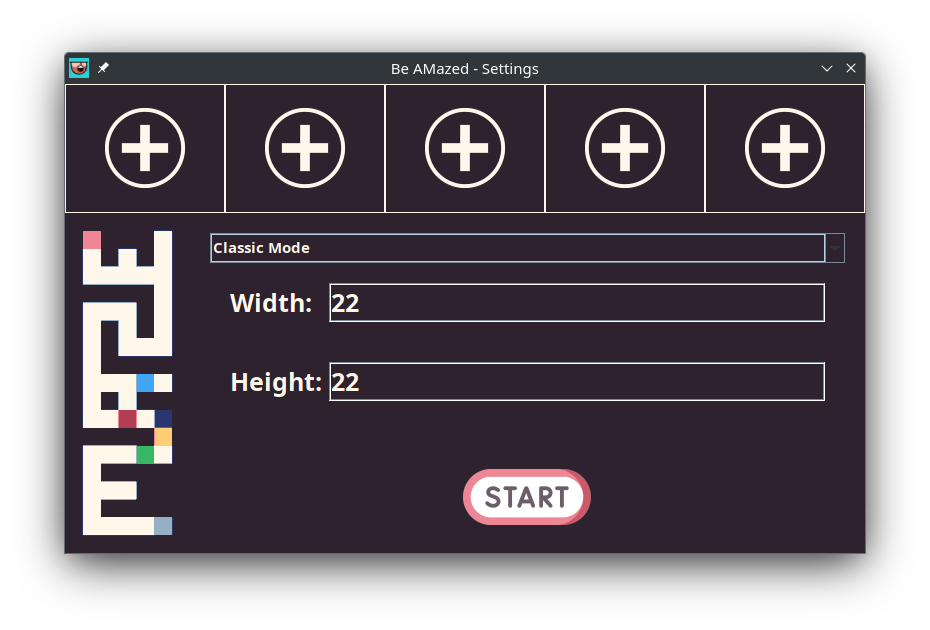
\includegraphics[width=10cm]{ressources/Implementation/Labyrinthe/Controleur/SettingsMenu_ClassicMode.png}
    \caption{Paramètres du mode classique}
    \label{fig:ClassicMode}
\end{figure}
\FloatBarrier

\subparagraph*{Le mode Blackout} (\ref{fig:BlackoutModeDifficulty})

Grâce à la classe \textbf{\textit{BlackoutPanelHandler}}, le mode Blackout possède 3 difficultés : \textbf{\textit{EASY}}, \textbf{\textit{MEDIUM}} et \textbf{\textit{HARD}} qu'on peut sélectionner grâce à un menu déroulant.

\begin{figure}[h!]
    \centering
    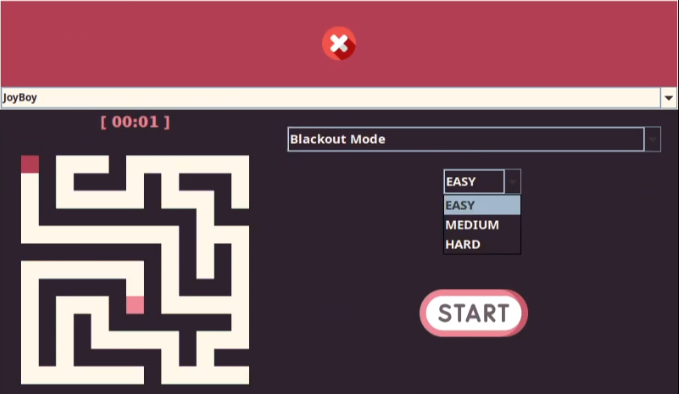
\includegraphics[width=10cm]{ressources/Implementation/Labyrinthe/Controleur/SettingsMenu_BlackoutMode_Difficulty.png}
    \caption{Paramètres du mode Blackout}
    \label{fig:BlackoutModeDifficulty}
\end{figure}
\FloatBarrier

\newpage

\subparagraph*{La préparation des joueurs} (\ref{fig:PlayerSelection})

Grâce aux classes \textbf{\textit{PlayerPanel}}, \textbf{\textit{PlayerSelectionPanel}} et \textbf{\textit{UserSelector}}, nous pouvons choisir le nombre de joueurs, leur couleur et leur nom parmi la liste des joueurs qui ont déjà été crées précédemment.

Tout d'abord, pour ajouter un joueur, on clique sur une case "+". Une case de couleur s'affichera. Ensuite on choisit le nom du joueur dans la liste déroulante. Enfin il faut confirmer que le joueur est prêt en cliquant sur sa case.

\begin{figure}[h!]
    \centering
    \begin{subfigure}{6.5cm}
        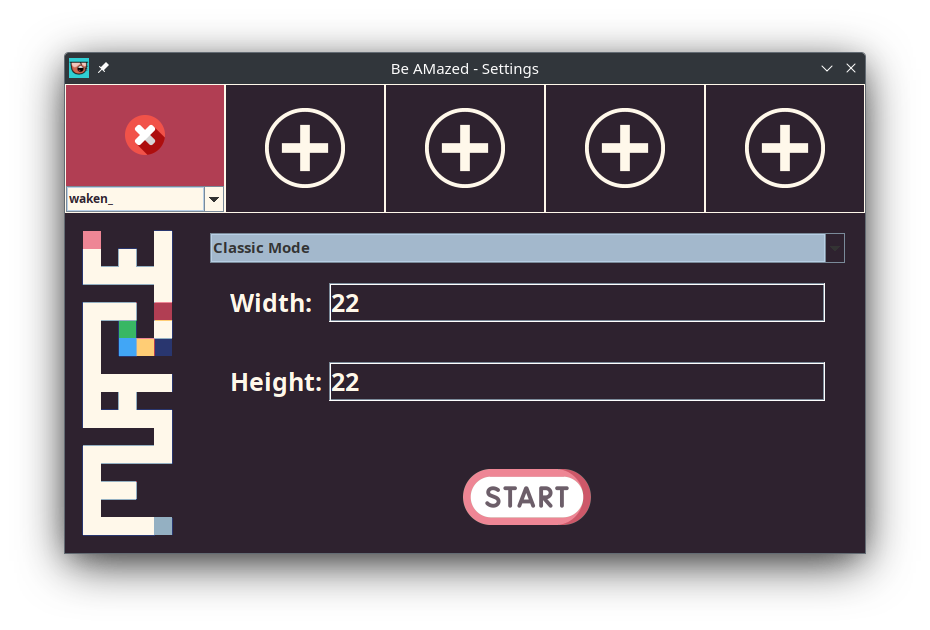
\includegraphics[width=6.5cm]{ressources/Implementation/Labyrinthe/Controleur/SettingsMenu_NotReady.png}%
        \caption{Joueur pas prêt}
        \label{fig:PlayerNotReady}
    \end{subfigure}
    \qquad
    \begin{subfigure}{6.5cm}
        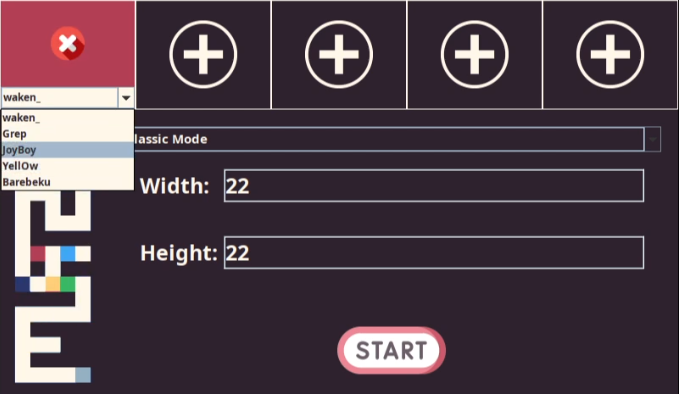
\includegraphics[width=6.5cm]{ressources/Implementation/Labyrinthe/Controleur/SettingsMenu_PlayerList.png}%
        \caption{Liste des joueurs disponibles}
        \label{fig:PlayersAvailable}
    \end{subfigure}
    \qquad
    \begin{subfigure}{6.5cm}
        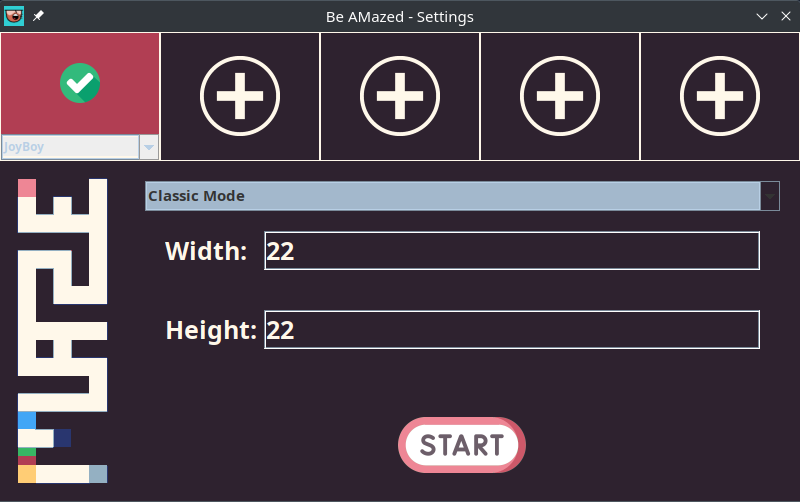
\includegraphics[width=6.5cm]{ressources/Implementation/Labyrinthe/Controleur/SettingsMenu_Ready.png}%
        \caption{Joueur prêt}
        \label{fig:PlayerReady}
    \end{subfigure}
    \caption{Ajout d'un joueur}
    \label{fig:PlayerSelection}
\end{figure}
\FloatBarrier

\paragraph{Lancement de la partie}

Pour lancer la partie on clique sur le bouton
\vcenteredinclude[height=5mm]{ressources/Implementation/Labyrinthe/Controleur/StartButton.png}
après que tous les joueurs soient prêts et que les paramètres précédents aient été choisis.









